\chapter{Introducción específica} % Main chapter title
\label{Chapter2}

%----------------------------------------------------------------------------------------
% Resumen de capitulo
%----------------------------------------------------------------------------------------

En el presente capítulo se describe el estado actual de algunas soluciones implementadas, y se elige una plataforma existente, que cumple con los requerimientos del trabajo como base. También, se presenta el estudio del código fuente de \textit{Arm Mbed OS Simulator}. 

%----------------------------------------------------------------------------------------
\section{Estado del arte}
\label{sec:Estado del arte}
%----------------------------------------------------------------------------------------

Hoy en día no existe una herramienta de emulación para la placa EDU-CIAA-NXP. Sin embargo, existe la plataforma de código abierto ViHard \citep{ViHard} que emula dispositivos de hardware en la PC, pero con la placa ECU-CIAA-NXP real conectada a la PC a través del puerto USB. En la figura \ref{fig:ViHard} se muestra el esquema de la plataforma ViHard.

\begin{figure}[ht]
	\centering
	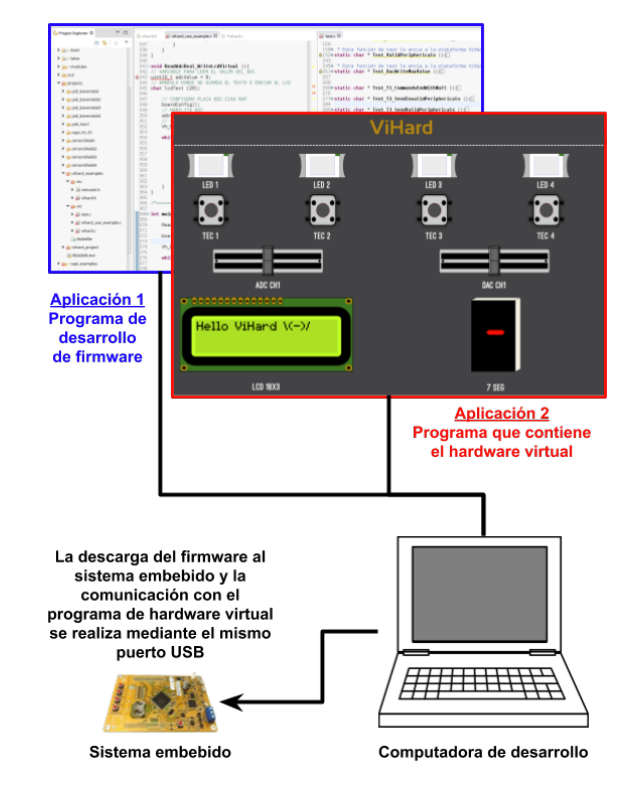
\includegraphics[scale=.40]{./Figures/ViHard.png}
	\caption{Esquema de la plataforma ViHard.\protect\footnotemark}
	\label{fig:ViHard}
\end{figure}

La plataforma se compone de un programa de PC con los perifericos virtuales de hardware y una biblioteca de firmware para la EDU-CIAA-NXP, que controla y gestiona el funcionamiento del hardware virtual. Ambos programas se comunican con el sistema embebido mediante UART, a través de un puerto USB.

El programa de hardware virtual es una aplicacion de escritorio multiplataforma desarrollada utilizando el framework Electron \citep{Electron}. Por otro lado, la biblioteca embebida fue desarrollada en lenguaje C. 

Por lo tanto, el usuario necesita ejecutar en su PC el programa de periféricos virtuales y contar con la biblioteca en el sistema embebido que controla el hardware virtual. A partir de ahí, procedería al desarrollo de su propio programa, que deberá compilar y descargar a la EDU-CIAA-NXP, y posteriormente realizar las pruebas correspondientes.

Por otro lado, se encontraron muchas plataformas educativas que simulan microcontroladores, sobre todo para la placa Arduino \citep{Arduino}. Para el análisis, se seleccionaron algunos de los simuladores más populares que implementan funcionalidades relevantes para el presente trabajo, los cuales se describen en las siguientes secciones. 

%------------------------------------
\subsection{UnoArduSim}

UnoArduSim \citep{UnoArduSim} fue desarrollado en la Universidad de Queen \citep{Queensu} por el profesor Stan Simmons. En la figura \ref{fig:UnoArduSim} puede observarse la interfaz del programa.

\begin{figure}[ht]
	\centering
	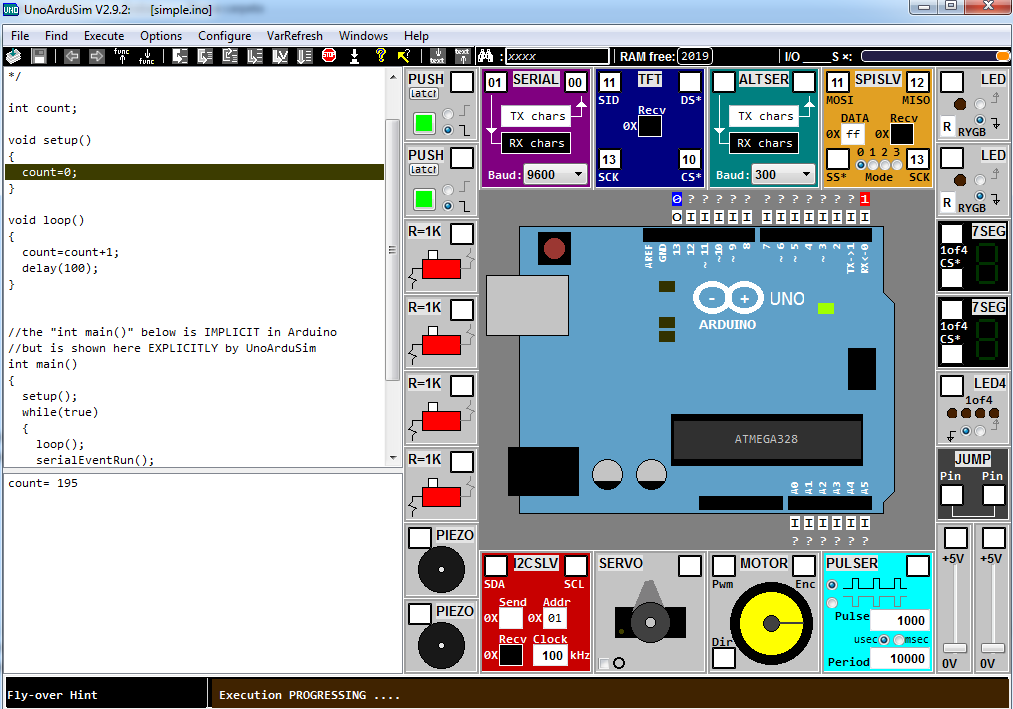
\includegraphics[scale=.33]{./Figures/UnoArduSim.png}
	\caption{Plataforma UnoArduSim.}
	\label{fig:UnoArduSim}
\end{figure}

La herramienta simula en la pantalla de la PC la placa Arduino Uno \citep{ArduinoUno} y muchos de los dispositivos de entrada y salida más usados, asimismo, permite la depuración interactiva de funciones o programas completos. Está diseñada específicamente para ejecutarse en el sistema operativo Windows. Además, el diseño de la interfaz gráfica no promueve la claridad visual, puesto que hay demasiados objetos en la pantalla y los que existen deberían estar mejor distribuidos. 

%------------------------------------
\subsection{Virtronics}

Virtronics \citep{Virtronics} es uno de los simuladores más completos que hay hoy en día para Arduino \citep{Arduino}, ya que permite simular varios modelos y, además, tiene dos versiones disponibles: una versión paga y otra gratuita, pero con funciones limitadas. En la figura \ref{fig:Virtronics} se muestra la plataforma.

\begin{figure}[ht]
	\centering
	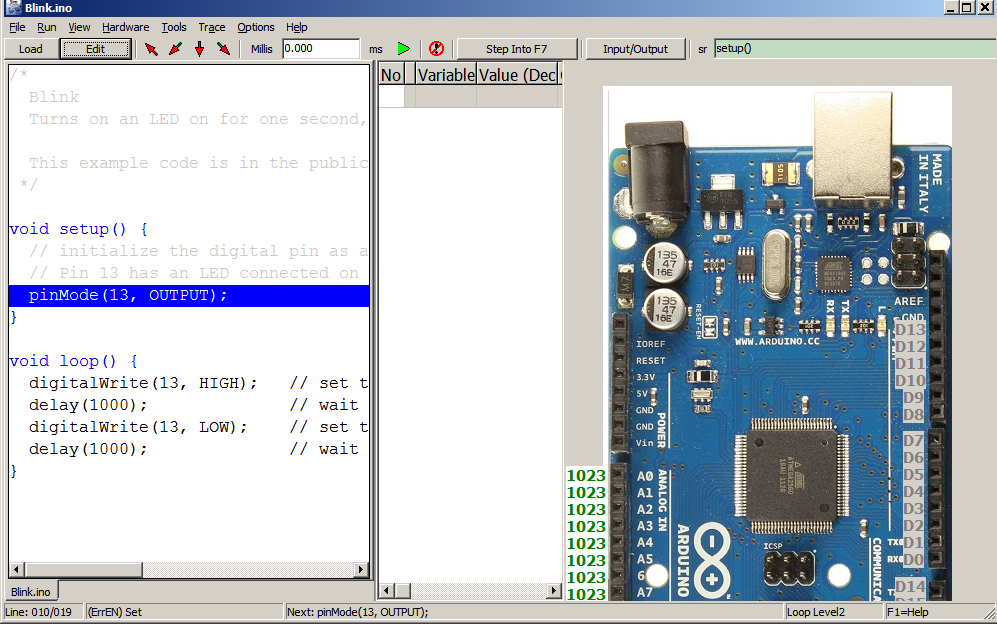
\includegraphics[scale=.35]{./Figures/Virtronics.png}
	\caption{Plataforma Virtronics.}
	\label{fig:Virtronics}
\end{figure}

%------------------------------------
\subsection{Tinkercad}

Tinkercad \citep{Tinkercad} es una plataforma online que permite el acceso desde cualquier navegador web, cuya interfaz de usuario se muestra en la figura \ref{fig:Tinkercad}.

\begin{figure}[ht]
	\centering
	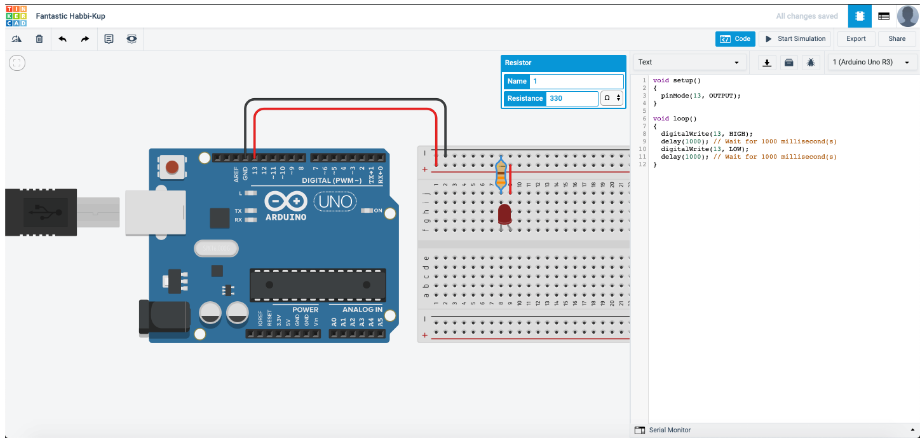
\includegraphics[scale=.40]{./Figures/Tinkercad.png}
	\caption{Plataforma Tinkercad.}
	\label{fig:Tinkercad}
\end{figure}

Fue desarrollado por ingenieros y diseñadores de software de Autodesk \citep{Autodesk} y permite diseños 3D. Adicionalmente, es necesario crear una cuenta  antes de empezar a usar la plataforma, por consiguiente, todos los diseños se guardan en la cuenta creada. 

%------------------------------------
\subsection{\textit{Arm Mbed OS Simulator}}

\textit{Arm Mbed OS Simulator} \citep{ArmMbedSim} fue desarrollado por ingenieros de Arm, encargados de mantener las bibliotecas Mbed OS, \citep{ArmMbed} y es parte de Mbed Labs. La plataforma era accesible \textit{on line} al momento del comienzo de este proyecto, pero actualmente debe ser descargado desde su repositorio \citep{ArmMbedSimRepo} y luego, puede ejecutarse utilizando cualquier navegador web en la red local, o bien, realizar el despliegue en un servidor para que esté disponible \textit{on line}. En la figura \ref{fig:ArmMbed} puede observarse la plataforma online de Mbed Simulator.

\begin{figure}[ht]
	\centering
	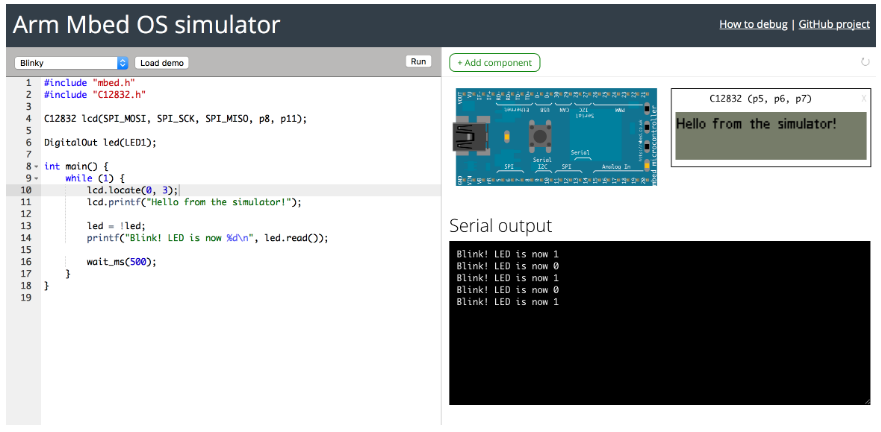
\includegraphics[scale=.44]{./Figures/ArmMbed.png}
	\caption{Plataforma Arm Mbed OS Simulator.}
	\label{fig:ArmMbed}
\end{figure}

El funcionamiento de este emulador es muy simple. Se puede crear un programa desde cero, o bien, se puede elegir un ejemplo de la lista desplegable y cargar el proyecto desde el botón \textquotedbl Load demo\textquotedbl, luego añadir los componentes necesarios para el programa, como por ejemplo, el display que se observa en la figura \ref{fig:ArmMbed}, donde se pide al usuario indicar a qué pines estará conectado. Es importante mencionar que el programa ya incluye la placa con el microcontrolador precargada. Una vez completo el programa y el ensamblado del hardware, se puede compilar y ejecutar en el emulador usando el botón \textquotedbl Run\textquotedbl.

%----------------------------------------------------------------------------------------
\section{Análisis de los emuladores revisados}
\label{sec:Análisis de los emuladores revisados}
%----------------------------------------------------------------------------------------

En la tabla \ref{tab:simuladores} se comparan las características más importantes de estos emuladores. 

\hfill \break
\hfill \break
\hfill \break
\hfill \break
\hfill \break
\hfill \break
\hfill \break
\hfill \break
\hfill \break

\begin{table}[ht]
\centering
\caption[Comparación de características de los emuladores revisados]{Comparación de características de los emuladores revisados}
\begin{tabular}{p{0.24\linewidth} p{0.17\linewidth}  p{0.19\linewidth}  p{0.14\linewidth}  p{0.10\linewidth}}
\toprule
\textbf{Característica} 
& \textbf{UnoArduSim}
& \textbf{Virtronics}
& \textbf{Tinkercad}
& \textbf{Mbed OS}
\\
\midrule
Placa/Plataforma emulada & Arduino Uno y Mega & Varios modelos Arduino & Arduino Uno & Arm Mbed OS\\
Gratuito &    Sí & No & Sí & Sí\\
Aplicación & Escritorio & Escritorio & Web & Web\\
Plataforma & Windows & Windows/Linux & Todas & Todas\\
Código abierto & No & No & No & Sí\\
Dispositivos E/S & Sí & Sí & Sí & Sí  \\
Panel de desarrollo & Sí & Sí & Sí & Sí \\
Lenguaje & C & C & C & C/C++\\
Debugging & Sí & Sí & Sí & No\\
Ejemplos & Sí & Sí & Sí & Sí\\
\bottomrule
\hline
\end{tabular}
\label{tab:simuladores}
\end{table}

Cabe destacar, que de las plataformas revisadas \textit{Arm Mbed OS Simulator} es la única de código abierto. Sin embargo, este análisis sirve tembién para revisar, comprender y comparar las ventajas y desventajas de las otras plataformas, y tomar características útiles para el desarrollo del emulador. 

Del análisis anterior, se desprende que \textit{Arm Mbed OS Simulator} presenta las siguientes ventajas significativas:

\begin{itemize}
	\item Código abierto: al tener acceso al código fuente permitió estudiar cómo funciona internamente el proyecto simulador, además, de la libertad de uso y distribución.
	\item Arquitectua de aplicación web. 
    \item Su capacidad para simular dispositivos y componentes.
	\item Comunidad y Soporte: el proyecto tiene una comunidad activa de desarrolladores, que brinda acceso a una amplia base de conocimientos, documentación y soporte. 
	\item Reconocimiento de Marca ARM mbed OS: al basarse en su proyecto simulador, se puede obtener cierto reconocimiento y confianza entre los usuarios.
	\item Reutilización: ofrece un conjunto sólido de funcionalidades y características ya probadas que agilizó el desarrollo y redujo la probabilidad de introducir errores.
	\item Actualizaciones y Mejoras Continuas: el proyecto Mbed Simulator recibe actualizaciones continuas con las últimas tecnologías que permite mantener el emulador para la placa EDU-CIAA-NXP actualizado.	
\end{itemize}

Sim embargo, actualmente, \textit{Arm Mbed OS Simulator} presenta las siguientes limitaciones:

\begin{enumerate}
	\item Dentro de un bucle infinito \texttt{while(1)}, es necesario agregar un retraso \newline(\texttt{delay)}, de lo contrario, el navegador no puede actualizar la interfaz de la plataforma web ni responder a eventos del usuario. Esto significa que el navegador no tiene la oportunidad de realizar otras tareas o responder a eventos mientras el bucle está en ejecución. Como resultado, el navegador se bloquea o congela y puede dejar de responder.
	
	\item En cada iteracion, la ejecución del programa puede variar en términos de tiempo, lo que puede afectar a la precisión en la sincronización de eventos dentro de la aplicación.

	\item En \textit{Arm Mbed OS Simulator}, no hay restricciones significativas en cuanto a la cantidad de memoria que se puede asignar al stack o al heap  de un programa, lo cual difiere del hardware físico, donde sí existen limitaciones de memoria.
	
	\item Dentro del entorno web, las interrupciones no se manejan de la misma manera que en un sistema embebido real, debido a que no implementa el manejo de prioridades, por lo cual no afectan la ejecución del programa principal.
	
	\item Sin RTOS. No tiene la capacidad de ejecutar múltiples hilos de manera concurrente como lo haría un RTOS. Todo el código se ejecuta en un solo hilo. Se puede utilizar la biblioteca mbed-events para manejar ciertos aspectos de concurrencia, usando eventos y temporizadores.
	
	\item Emulación a nivel API de Mbed OS. No permite programar a bajo nivel, utilizando registros de core para la arquitectura ARM o periféricos.
	
	\item Sin capacidad de debug paso a paso. Se realiza el programa, se compila y ejecuta en el hardware virtual pero no permite la depuración de código.
\end{enumerate}

Dadas todas estas consideraciones y una vez confirmada su compatibilidad para los propósitos del presente trabajo, se decide basar el emulador de la EDU-CIAA-NXP en portar el proyecto \textit{Arm Mbed OS Simulator}, para la EDU-CIAA-NXP y sus bibliotecas.

%----------------------------------------------------------------------------------------
\section{Análisis de \textit{Arm Mbed OS Simulator}}
%----------------------------------------------------------------------------------------

Se procedió a analizar en detalle el código fuente de \textit{Arm Mbed OS Simulator} para adquirir una compresión de su arquitectura, del funcionamiento del \textit{Sistema Operativo Mbed}, de los periféricos simulados y sus las interacciones, así como de las configuraciones necesarias para la plataforma web.

%------------------------------
\subsection{Tecnologías utilizadas}
\label{sec:Tecnologías utilizada}

\textit{Arm Mbed OS Simulator} es una aplicación web. Este tipo de aplicaciones son provistas por un servidor web y pueden ser accedidas por los usuarios que se conecten a través de internet desde cualquier lugar mediante un navegador web \citep{NavegadorWeb}. Las aplicaciones web se basan en una arquitectura cliente/servidor (figura \ref{fig:ClienteServidor}), en donde un cliente o navegador web realiza peticiones al servidor y en consecuencia el servidor envía la respuesta de regreso.

\begin{figure}[ht]
	\centering
	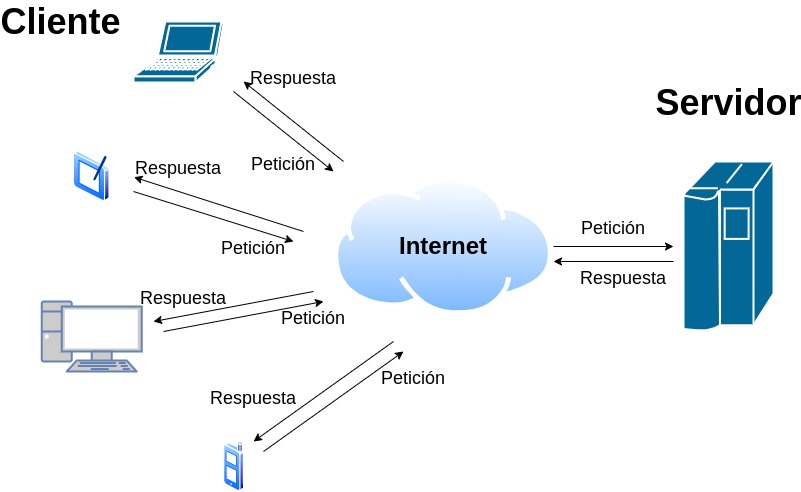
\includegraphics[scale=.48]{./Figures/EsquemaCliente_Servidor.jpg}
	\caption{Esquema modelo cliente/servidor.}
	\label{fig:ClienteServidor}
\end{figure}

\hfill \break
\hfill \break
\hfill \break

Las ventajas más importantes que presenta la tecnologia web son:

\begin{itemize}
	\item No es necesario instalar nada en la computadora del usuario.
	\item Muy bajo consumo de recursos del lado del cliente, la mayor carga se encuentra del lado del servidor.
	\item Es posible acceder al emulador desde cualquier ubicación con una conexión a internet.
	\item El usuario no requiere tener un sistema operativo específico, ya que se puede ejecutar en todos los dispositivos con acceso a un navegador web y una conexión a internet.
\end{itemize}

\textit{Arm Mbed OS Simulator} está desarrollado principalmente sobre las siguientes tecnologías:

\begin{itemize}

    \item \textit{Node.JS} \citep{NodeJS}: es un entorno de ejecución del lenguaje de programación \textit{JavaScript} \citep{JavaScript} cuyo propósito es el desarrollo de aplicaciones web y servicios del lado del servidor. También, proporciona una arquitectura orientada a eventos y no bloqueante. 
 
    \item \textit{Emscripten} \citep{Emscripten}: es una \textit{toolchain} de compilación completo para \textit{WebAssembly}, que utiliza \textit{LLVM} \citep{LLVM}) y \textit{Binaryen} \citep{Binaryen}, para compilar C y C++ en \textit{WebAssembly} \citep{WebAssembly} y \textit{JavaScript}. La salida de \textit{Emscripten} puede ejecutarse en la web y en \textit{Node.JS}. Esto permite ejecutar aplicaciones desarrolladas en C y C++ en la web, sin necesidad de plugins o complementos adicionales.

    \item \textit{Arm Mbed OS} \citep{MbedOS}: es un sistema operativo para sistemas embebidos, de de código abierto, diseñado específicamente para los dispositivos \textit{IoT}. Incluye todas las funciones que necesita para desarrollar un producto conectado, basado en un microcontrolador \textit{Arm Cortex-M}, incluida seguridad, conectividad, \textit{RTOS} y controladores para sensores y dispositivos de Eentrada/Salida.
    
    \item \textit{Arm Mbed CLI} \citep{MbedCLI}: es una herramienta de línea de comandos que facilita el desarrollo y la gestión de proyectos basados en la plataforma \textit{Arm Mbed OS}, permite realizar tareas como la configuración del entorno de desarrollo, compilación de código, gestión de dependencias y la depuración, además, de identificar y resolver problemas en el código.

\end{itemize}

%------------------------------
\subsection{Descirpción funcional básica}

Estas tecnologías presentadas en la sección \ref{sec:Tecnologías utilizada} se relacionan entre sí como se meustra en la figura \ref{fig:AsiFuncionaMbedSim}.

\begin{figure}[ht]
	\centering
	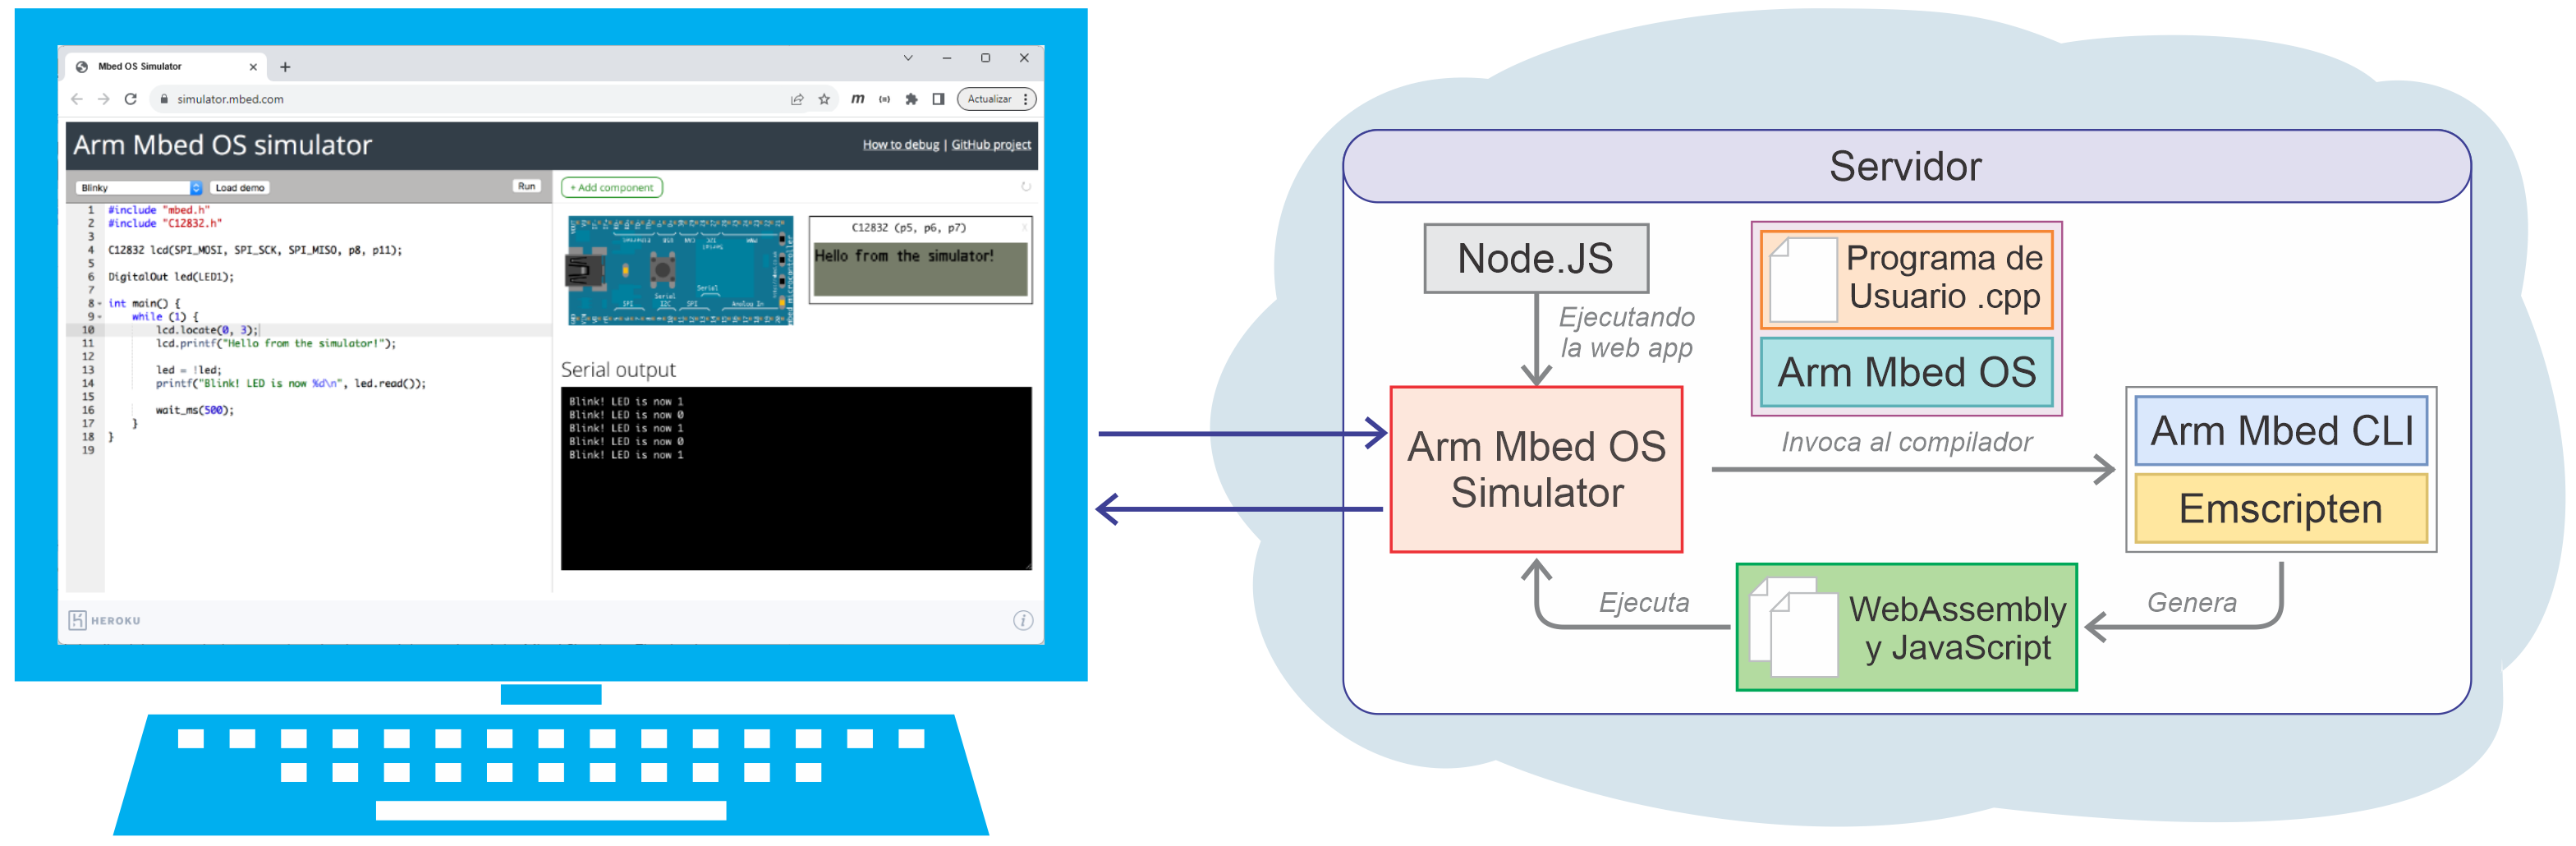
\includegraphics[scale=.52]{./Figures/funcionamientoMbed.png}
	\caption{Funcionamiento de \textit{Arm Mbed OS Simulator}.}
	\label{fig:AsiFuncionaMbedSim}
\end{figure}

\textit{Node.JS} ejecuta \textit{Arm Mbed OS Simulator} dentro un servidor web. Un usuario puede accedear a la aplicación web mediante un navegador web para utilizarla. 

Cuando el usuario finaliza el programa en C/C++ y el ensamblado del hardware, puede proceder a presionar el botón \textit{Run} para compilar y ejecutar el programa. En este proceso, se integra el programa de usuario con la biblioteca \textit{Arm Mbed OS}. Posteriormente, se compila todo en conjunto mediante las herramientas \textit{Emscripten} y \textit{Arm Mbed CLI}.

El resultado de dicha compilación, el es mismo programa en \textit{WebAssembly} y \textit{JavaScript}, que luego se ejecuta sobre el hardware virtualizado, permitiendole al usuario probar su funcionamiento.

%------------------------------
\subsection{\textit{Frontend} y \textit{Backend}}

En el contexto del desarrollo de aplicaciones web, se denomina \textit{Frontend} a la interfaz que los usuarios interactúan directamente, siendo la cara visible del sitio en el lado del cliente. Por otro lado, el \textit{Backend} es la parte lógica que se encarga de la conexión con el servidor, de tomar los datos, procesarlos y devolverlos al \textit{Frontend}.

En la figura \ref{fig:FrontendBackendMbed} se muestra un esquema con las tecnologías utilizados tanto en el \textit{Frontend} como en el \textit{Backend} de \textit{Arm Mbed OS Simulator}.

\begin{figure}[ht]
	\centering
	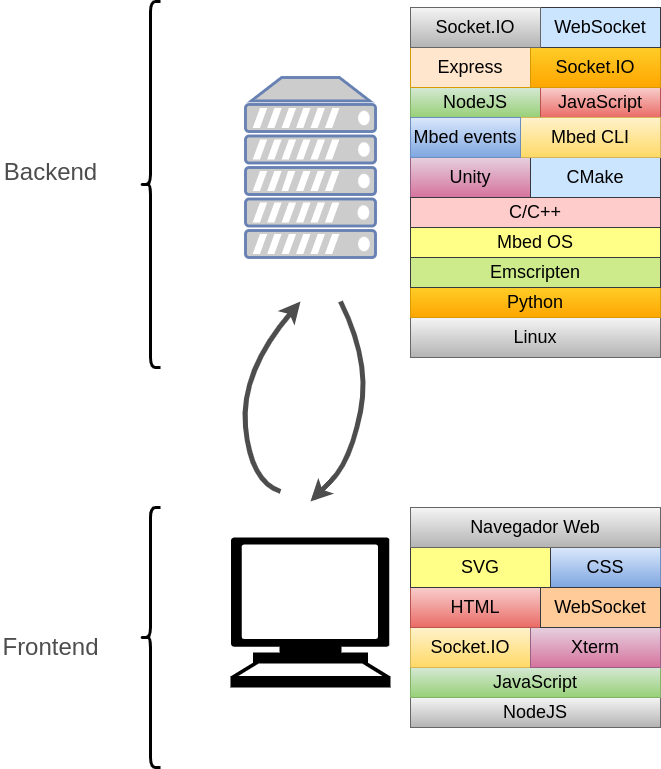
\includegraphics[scale=.47]{./Figures/FrontendBackendMbed.png}
	\caption{Esquema de las tecnologías utlilizadas en \textit{Arm Mbed OS Simulator}.}
	\label{fig:FrontendBackendMbed}
\end{figure}

\newpage

Como se puede observar, existen tecnologías que utilizan en ambas partes de la aplicación y otras correspondientes únicamente al \textit{Frontend}, o al \textit{Backend}.

El lenguaje de programación \textit{JavaScript} del lado del cliente, permite crear páginas web dinámicas y también responder a eventos causados por el propio usuario tales como modificaciones del DOM (siglas en inglés de \textit{Document Object Model} \citep{DOM}). Por consiguiente, en el \textit{frontend} permite cargar y ejecutar los archivos resultantes generados por el compilador en el navegador. Asimismo, es el responsable de configurar el entorno necesario para ejecutar la aplicación web y proporcionar la interfaz de usuario para la interacción. 

En el \textit{backend}, \textit{JavaScript} se utiliza para gestionar la comunicación y la interacción entre los diferentes componentes a través de solicitudes HTTP, permitiendo la transferencia de datos y el flujo de información dentro de la plataforma web.

Los paquetes de \textit{Node.JS} consisten en es uno o más archivos \textit{.js} o \textit{.ts} (módulos) agrupados (o empaquetados) juntos. Los archivos en un paquete son código reutilizable que realiza una función específica en la aplicación \textit{Node.JS}. \textit{Arm Mbed OS Simulator} utiliza los siguientes paquetes:

\begin{itemize}
    \item En \textit{Frontend} y \textit{Backend}:
        \begin{itemize}
    	\item \textit{socket.io}
    	\item \textit{timesync}
        \end{itemize}
    \item Solo en \textit{Frontend}
        \begin{itemize}
            \item \textit{xterm}
        \end{itemize}
    \item Solo en {Backend}:
        \begin{itemize}
            \item \textit{body-parser}
            \item \textit{express}
            \item \textit{command-exists}
            \item \textit{commander}
            \item \textit{compression}
            \item \textit{es6-promisify}
            \item \textit{getmac}
            \item \textit{hbs}
            \item \textit{opn}
            \item \textit{puppeteer}
        \end{itemize}
\end{itemize}

Se describen los paquetes más relevantes:

\begin{itemize}
    \item \textit{Socket.IO} \citep{Socket}: es un paquete que utiliza \textit{websockets} para comunicación bidireccional con baja latencia. La plataforma, utiliza \textit{Socket.IO} para establecer la comunicación entre el \textit{Frontend} y el \textit{Backend}, y de esta manera, permitir la transferencia de datos de manera dinámica con el fin de actualizar los eventos entre ambas partes de la plataforma.

    \item \textit{Xterm} \citep{Xterm}: es un paquete escrito en \textit{TypeScript} \citep{TypeScript} para el que permite que una aplicación pueda usar terminales emuladas con todas sus funciones en el navegador web (\textit{Frontend}). La plataforma web utiliza esta tecnología en la interfaz de usuario para visualizar la salida de la UART de la placa simulada en una terminal serie.

    \item \textit{Express} \citep{Express}: es un marco de aplicaciones web en el \textit{Backend} para \textit{Node.JS} diseñado para crear aplicaciones web y APIs (siglas en inglés de \textit{application programming interface}) \citep{API}. Se utiliza \textit{Express} para configurar \textit{middlewares} que permiten servir archivos estáticos desde carpetas específicas, como \textquotedbl \textit{out} \textquotedbl, que contiene los archivos generados por \textit{Emscripten}.

\end{itemize}

Tecnologías que se utilizan solamente en el \textit{frontend} de \textit{Arm Mbed OS Simulator}:

\begin{itemize}
    \item HTML \citep{HTML}: son las siglas en inglés de \textit{HyperText Markup Language}, o en español, Lenguaje de Marcas de Hipertexto. Es un lenguaje de marcado que permite la estructuración de información y contenido en un documento o sitio web. El marcado se ejecuta a través de etiquetas que cumplen diferentes funciones en la estructuración del documento paravisualizarlos en el navegador web.
    Este lenguaje es sencillo de aprender y es fácil de  tanto por humanos como por máquinas. Se utiliza para definir el contenido de la interfaz de usuario, como los botones, lista desplegable, pantallas de visualización, y otros componentes necesarios para interactuar con la plataforma web.

    \item SVG \citep{SVG}: de las siglas en inglés \textit{Scalable Vector Graphics}, es un estándar web para definir imágenes vectoriales bidimensionales. Las imágenes creadas con este formato se pueden escalar y hacer zoom de forma arbitraria sin pérdida de resolución debido a que, en lugar de estar formádos por píxeles, como otros formatos de imagen, son descriptos en base a objetos como líneas, círculos y poligonos, entre otros. Este tipo de gráficos se describe mediante un archivo de texto cuya estructura está basada en el lenguaje de marcado extensible \textit{XML} \citep{XML}, siendo un formato muy útil para ser utilizado en entornos web. Este tipo de gráficos se utiliza en la plataforma para representar gráficamente la placa de desarrollo donde se ejecutan los programas, y permitir interactuar con su botón y LED.

    \item CSS \citep{CSS}: de las siglas en inglés \textit{Cascading Style Sheets}, es un lenguaje de diseño gráfico que permite definir estilos, colores, formato, tamaño, tipo de letra del texto, posición de cada elemento dentro dentro de la pantalla en una páhina HTML o imagen SVG. Es la mejor forma de separar los contenidos de su diseño, y es necesario para crear páginas web complejas. De esta manera, CSS controla la presentación visual y el estilo del contenido HTML y SVG de esta plataforma web.

    \item Imágenes: se utilizan imágenes \textit{.png} de los LEDs virtuales a conectar con la placa virtual.

\end{itemize}

Finalmmente, se describen las tecnologías se utilizan solamente en el \textit{Backend} de \textit{Arm Mbed OS Simulator}:

\begin{itemize}

    \item \textit{Python} \citep{Python}: es un poderoso y popular lenguaje de programación multiplataforma, de código abierto, y un entorno de ejecución. Se caracteriza por su sencillez y su gran potencia para el tratamiento de datos en el lado del servidor. En la plataforma web, \textit{Python} 2.7 se utiliza para ejecutar scripts que realizan tareas específicas, como la configuración e inicialización y la ejecución de \textit{Arm Mbed CLI}.

    \item Lenguajes C / C++ \citep{LenguajeC}: son lenguajes de propósito general y muy populares debido al eficiente código que produce al crear software de sistemas y de aplicaciones.  Las bibliotecas \textit{Arm MBed OS} y los programas que el usuarrio desarrolla para la placa virtual, están escritos en estos lenguajes.

    \item \textit{Mbed events} \citep{ArmMbedEvents}: es una biblioteca de código escrita en lenguaje C que se utiliza en el desarrollo de software embebido para facilitar la gestión de eventos y temporizadores. Para el desarrollo de la plataforma usa esta biblioteca para la creación y gestión de tareas en el \textit{RTOS}. Aunque su uso no permite obtener las funcionalidades requeridas.
    
\end{itemize}

%------------------------------
\subsection{Descipción funcional en detalle}

En el diagrama de bloques de la figura \ref{fig:Arquitectura} se muestra la arquitectura básica de una aplicación de usuario que ejecuta en \textit{Arm Mbed OS Simulator} y las capas de software involucradas.

\begin{figure}[ht]
	\centering
	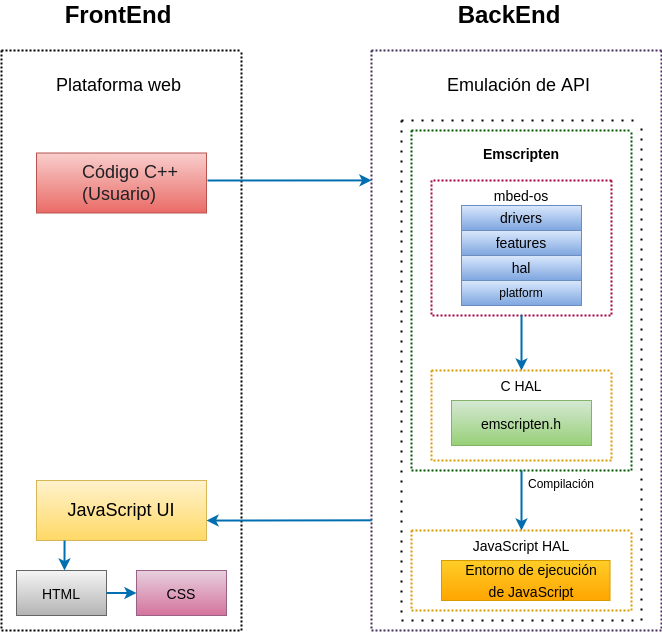
\includegraphics[scale=.55]{./Figures/ArquitecturaMBED.png}
	\caption{Arquitectura de capas de la plataforma \textit{Arm Mbed OS Simulator}.}
	\label{fig:Arquitectura}
\end{figure}

\newpage

\textit{Arm Mbed OS Simulator} presenta una emulación a nivel de API de la biblioteca \textit{Mbed OS} debido a que gran parte de las API son genéricas entre diferentes plataformas de hardware objetivo soportadas (en inglés, \textit{targets}). Esto incluye las capas de periféricos, como GPIO, \textit{stacks} de redes IP4/IPV6 y bibliotecas de comunicación como \textit{CoAP} o \textit{LoRaWAN}. El código específico del \textit{target}, como, por ejemplo, en qué registros escribir para cambiar el valor de pin GPIO, se implementa utilizando la capa \textit{Mbed C HAL}. \textit{HAL} son las siglas en inglés de \textit{Hardware Abstaction Layer}, en español, capa de abstacción de hardware. De esta manera, para implementar el \textit{port} de la biblioteca \textit{Arm Mbed OS} a una nueva plataforma de hardware, solamente se deben portar los archivos pertenecientes a la capa \textit{Mbed C HAL}.

\textit{Arm Mbed OS Simulator} utiliza el mismo enfoque, implementando un nuevo \textit{target}, nombrado (TARGET\_SIMULATOR) que implementa la capa \textit{Mbed C HAL}. Sin embargo, la diferencia más importante, es que la capa \textit{Mbed C HAL} que implementa en \textit{Arm Mbed OS Simulator}, en lugar de escribir registros de un microcontrolador real, pasa eventos a una \textit{HAL} implementada en JavaScript (nombrada capa \textit{JS HAL}). Luego, la interfaz de usuario se suscribe a estos eventos y actualiza en consecuencia los componentes gráficos del simulador, esto se implementa en una capa nombrada \textit{JS UI}).

Si se toma por ejemplo, un elemento la API \textit{DigitalOut} de \textit{Mbed OS}, el flujo de la información para controlar un \textit{LED} conectado a un pin configurado como salida es el que se describe en la figura \ref{fig:flujoGpio-LedMbed}.

\begin{figure}[ht]
	\centering
	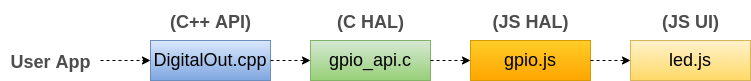
\includegraphics[scale=.50]{./Figures/flujoGpio-LedMbed.png}
	\caption{Ejemplo de flujo de información de pin de salida controlando un led en \textit{Arm Mbed OS Simulator}.}
	\label{fig:flujoGpio-LedMbed}
\end{figure}

Para que \textit{Mbed C HAL} pueda pasar los  eventos a la capa \textit{JS HAL} se utiliza la biblioteca \textit{emscripten.h}. Esta biblioteca provee las funciones y macros necesarias para interactuar con el compilador de \textit{Emscripten}, permitiendo que el código \textit{C} use funciones nativas \textit{JavaScript}. De esta manera, cuando se compila el programa de usuario, junto a \textit{Arm Mbed OS} con \textit{Emscripten} se obtienen archivos \textit{WebAssembly} y \textit{Javascrtipt} que pueden comunicarse con la capa \textit{JS HAL}.

La capa (\textit{JS HAL}) actúa como intermediario, distribuyendo eventos entre los componentes de las capas \textit{JS UI} y \textit{C HAL}. Para relizarlo, implementa un bus de eventos para permitir que la interfaz de usuario se suscriba a eventos de C++.
Para lograr este objetivo se utiliza la clase \textit{EventEmitter} del paquete \textit{Events} de \textit{Node.JS}. \textit{EventEmitter} monitoriza y activa los eventos, facilitando la interacción del navegador con el código \textit{JavaScript} y permitiendo la actualización de la interfaz de usuario de manera flexible y eficiente. 

\textit{EventEmitter} se basa en el modelo de publicación/suscripción que se trata de un paradigma de envío de mensajes asíncrono mediante el cual un usuario publica mensajes y uno o varios objetos se suscriben a esos eventos.

En la figura \ref{fig:PublicarSuscribir} se muestra el modelo de \textit{publicación/suscripción}.

\begin{figure}[ht]
	\centering
	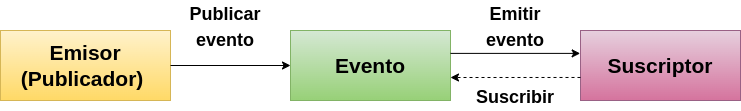
\includegraphics[scale=.49]{./Figures/PublicarSuscribir.png}
	\caption{Modelo de \textit{publicación/suscripción}.}
	\label{fig:PublicarSuscribir}
\end{figure}

Laos objetos de la capa \textit{JS UI} manejan los eventos de la interfaz de usuario y solo se comunica con \textit{JS HAL}. Para enviar cambios desde la inrefaz gráfica a la capa \textit{JS HAL}, se utiliza directamente su API, mientras que para recibir cambios en la interfaz gráfica desde la capa \textit{JS HAL}, los objetos de la capa \textit{JS UI} se sucriben al detector de eventos. 

Para describir este funcionamiento de la suscripción a los eventos, se debe introducir el concepto de \textit{listeners} (en español, oyentes) de \textit{JavaScript}. Los \textit{listeners} se crean utilizando el método \texttt{on()} y pasando como argumento el nombre del evento al que se quiere suscribir. 

La figura \ref{fig:EventemitterNodeJSUI} muestra que cuando se emite algún evento en la \textit{JS HAL}, entonces el oyente suscrito a ese evento en esta capa \textit{JS UI} lo podrá escuchar y realizar las acciones que correspondan para la funcionalidad requerida. 

\begin{figure}[ht]
	\centering
	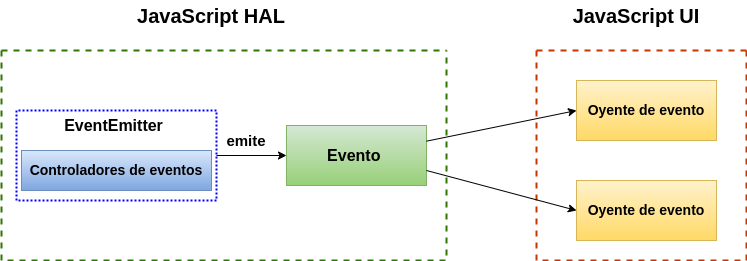
\includegraphics[scale=.52]{./Figures/EventemitterNodeJSUI.png}
	\caption{Diagrama de bloques de los oyentes de \textit{EventEmitter} en la capa UI.}
	\label{fig:EventemitterNodeJSUI}
\end{figure}

\newpage

De esta manera, existen varios subscriptores para un mismo evento en diferentes archivos \textit{JavaScript}. En consecuencia, se logra una mayor interactividad entre los componentes de la plataforma.

En resumen, se explica cómo un programa escrito en lenguaje \textit{C/C++} interactúa con la capa de abstracción de la emulación a nivel de API hasta llegar a la interfaz de usuario en \textit{JavaScript} para interactuar con los componentes de hardware virtuales, ya sea de la placa de desarrollo, o de componentes externos. 

%---------------------------------
\subsection{Caso de estudio: programa que activa un LED en la placa virtual}
\label{sec:caso_de_estudio}

Para exhibir el funcionamiento de \textit{Arm Mned OS} en su totalidad, se presenta en esta sección, un caso de estudio, correspondiente a la ejecución de un programa que activa un LED en la placa virtual.

El usuario escribe un programa en lenguaje \textit{C++}, que utiliza la biblioteca \textit{\textbf{Arm Mbed OS}} para interactuar con un pin configurado como salida, conectado a un \textit{LED}, ubicado en la propia placa virtual. 

A continuación, ejecuta el programa dentro de la plataforma web. Para lograr esto, mediante \textit{Node.js} se ejecutan los comandos necesarios para que \textit{Emscripten} realice la compilación del código \textit{C++}, que incluye: 

\begin{itemize}
    \item El codigo de la aplicacion de usuario escrito en lenguaje \textit{C++}.
    \item La biblioteca \textit{Arm Mbed Os}, capa \textit{Bibioteca C++}.
    \item El archivo \texttt{gpio\_api.c} de la capa \textit{C HAL}.
    \item El archivo \texttt{emscripten.h}.
\end{itemize} 

El proceso de compilación comienza con el preprocesamiento del código \textit{C++}, que incluye el manejo de directivas del preprocesador como \texttt{\#include} y \texttt{\#define}. Luego, el compilador utiliza \textit{LLVM} para compilar el código \textit{C} en \texttt{bitcode}. Después, de obtener el \texttt{bitcode} realiza optimizaciones para mejorar el rendimiento y reducir el tamaño del código resultante. Finalmente, \textit{Emscripten} toma el bitcode optimizado y lo traduce a código \textit{WebAssembly} y \textit{JavaScript}, permitiendo que el programa escrito originalmente en \textit{C++} pueda ser ejecutado dentro del entorno web. Los archivos resultantes de este proceso incluyen: 

\newpage

\begin{itemize}
    \item \texttt{user\_tiempoenmilisegundos.js}.
    \item \texttt{user\_tiempoenmilisegundos.wasm}.
    \item \texttt{user\_tiempoenmilisegundos.wast}.
    \item \texttt{user\_tiempoenmilisegundos.js.components}.
    \item \texttt{user\_tiempoenmilisegundos.wasm.map}.
\end{itemize}

\textit{Emscripten} utiliza un identificador único para los archivos generados. Este identificador esta compuesto por el prefijo \texttt{user\_} y un número entero que representa el tiempo en milisegundos.

Una vez que los archivos \texttt{.js} y \texttt{.wasm} se han generado a partir del código \textit{C++} mediante \textit{Emscripten}, pueden interactuar con el código \textit{JavaScript} de los archivos en las capas \textit{JS HAL} y \textit{JS UI}.

La figura \ref{fig:DiagramaSecuenciaMBED} muestra un diagrama de secuencia que expone la interacción del usuario con el sistema y sus capas interiores.

\begin{figure}[ht]
	\centering
	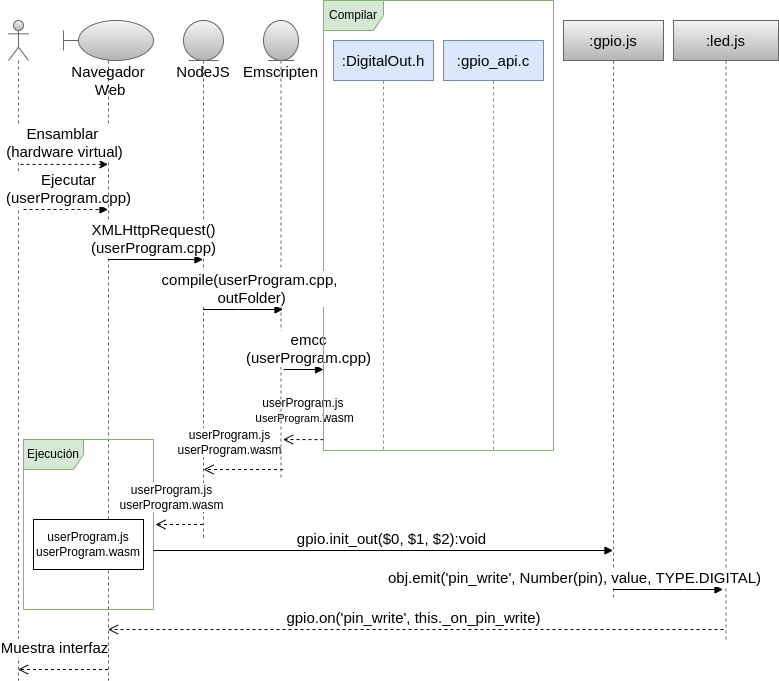
\includegraphics[scale=.49]{./Figures/DiagramaSecuenciaMBED.png}
	\caption{Funcionamiento de \textit{Arm Mbed OS Simulator}.}
	\label{fig:DiagramaSecuenciaMBED}
\end{figure}

La capa \textit{JS HAL} se encarga de notificar los eventos ocurridos. Mediante la función \texttt{write}, se realiza la activación del evento que escribe en el GPIO. 
Como resultado, emitirá el evento con el nombre \texttt{pin\_write}, pasando como argumentos el número de pin, el valor digital y el tipo de pin declarado, como se muestra en el diagrama en bloques de la figura \ref{fig:GPIOEventEmitter}.

\begin{figure}[ht]
	\centering
	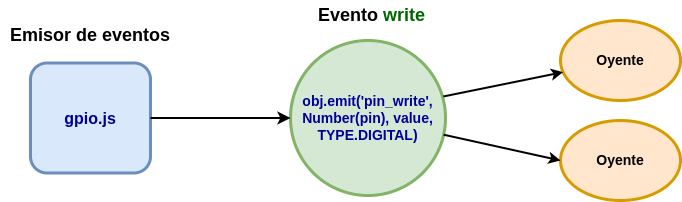
\includegraphics[scale=.55]{./Figures/GPIOEventEmitter.png}
	\caption{Activación de evento con el nombre \texttt{pin\_write}.}
	\label{fig:GPIOEventEmitter}
\end{figure}

En la capa \textit{JavaScript UI} cuando se emite el evento con el nombre \texttt{gpio\_write}, cualquier oyente que esté suscrito a ese evento podrá escucharlo y realizar las acciones correspondientes para la funcionalidad que se requiere. En este caso, la acción solicitada es encender el LED. Esto se ilustra en el diagrama en bloques de la figura \ref{fig:ListeningGPIOEventEmitter}.

\begin{figure}[ht]
	\centering
	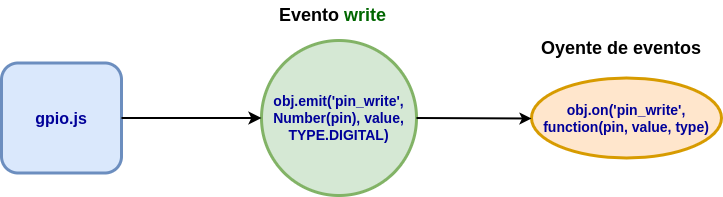
\includegraphics[scale=.50]{./Figures/ListeningGPIOEventEmitter.png}
	\caption{GPIO oyente del evento con el nombre \texttt{pin\_write}.}
	\label{fig:ListeningGPIOEventEmitter}
\end{figure}

Mediante estas interacciones entre todas las capas de programación, se muestrarán los cambios de \texttt{gpio\_write} en la placa virtual. Esto se resume en la figura \ref{fig:AplicacionUsuarioLeds}.

\begin{figure}[ht]
	\centering
	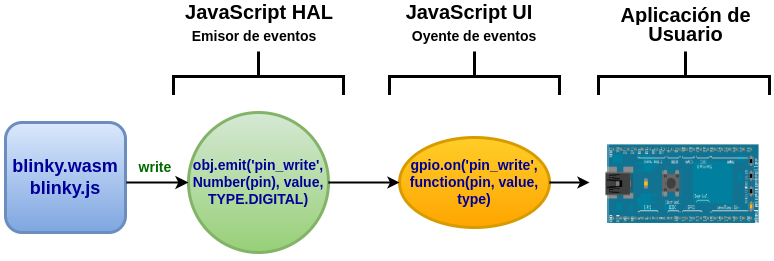
\includegraphics[scale=.62]{./Figures/AplicacionUsuarioLeds.png}
	\caption{Interacción entre todas las capas de programación.}
	\label{fig:AplicacionUsuarioLeds}
\end{figure}

%------------------------------
\subsection{Análisis estructural de archivos y carpetas}

En la figura \ref{fig:estructuraMbed1} se exhibe la estructura de arbol de las carpetas y archivos de \textit{Arm Mbed OS Simulator} al momento que fue clonado desde \textit{GitHub} para la realización de este trabajo.

\begin{figure}[ht]
	\centering
	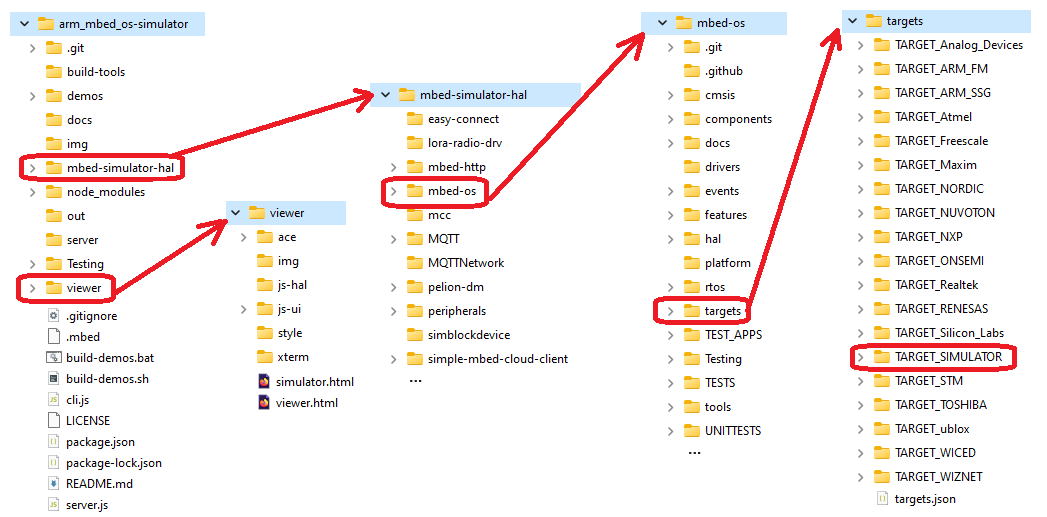
\includegraphics[scale=.50]{./Figures/carpetasYArchivosMbedOS.png}
	\caption{Estructura de carpetas y archivos de \textit{Arm Mbed OS Simulator}.}
	\label{fig:estructuraMbed1}
\end{figure}

\newpage

La carpeta \textquotedbl build-tools\textquotedbl{} contiene tres archivos \textit{javaScript}: 

\begin{enumerate}
    \item \textit{build-application.js}, que contiene funciones para construir aplicaciones en el contexto de \textit{Arm Mbed OS Simulator}. Asimismo, contiene métodos para encontrar los periféricos y manejar la construcción de componentes.
	
    \item \textit{build-libmbed.js}, es un módulo de la aplaicación web que realiza la compilación (\textit{(build)}) y gestión de dependencias.

    \item \textit{helpers.js}, es un módulo de la aplaicación web que proporciona funciones relacionadas con operaciones de sistema de archivos, compilación, y manipulación de directorios y archivos.
\end{enumerate}
 
Dentro de la carpeta \textquotedbl demos\textquotedbl{} se encuentran todos los programas ejemplo que el usuario puede seleccionar en \textit{Arm Mbed OS Simulator}. Estos están escritos en C/C++ y se utilizan como ejemplos didácticos que utilizan algunas de las funcionalidades de \textit{Arm Mbed OS}.
 
La carpeta \textquotedbl \textit{server}\textquotedbl{} contiene tres archivos \textit{JavaScript}: 

\begin{enumerate}
    \item \textit{compile.js}, este archivo realiza la generación de los archivos de salida compilados a partir del codigo fuente.

    \item \textit{get\_ips.js}, proporciona una función para la configuración de las aplicaciones de red.

    \item \textit{launch-server.js}, define y configura un servidor web que permite ejecutar solicitudes de ejecución de aplicaciones, gestionar las conexiones de red y la comunicación LoRaWAN.	
\end{enumerate}
 
La carpeta \textquotedbl viewer\textquotedbl{} contiene los archivos necesarios para crear interacción con el navegador en el \textit{Frontend}. Dentro de esta carpeta, se incuye:

\begin{itemize}
    \item Carpeta \textit{ace}: es un editor de código independiente escrito en \textit{JavaScript}. El objetivo es crear un editor de código basado en web que coincida y amplíe las características, la facilidad de uso y el rendimiento de los editores nativos existentes, como TextMate, Vim o Eclipse. 
    \item Carpeta \textit{img}: contiene imágenes \textit{.png} y \textit{.svg} utilizadas para describir los LEDs y la placa dde desarrollo respectivamente.
    \item Carpeta \textit{js-hal}: incluye todos los archivos que implementan la capa de abstracción de hardware en \textit{JavaScript}, o \textit{JavaScript HAL}.
    \item Carpeta \textit{js-ui}: incluye todos los archivos que implementan los componentes de interfaz de usuario en \textit{JavaScript}, nombrado \textit{JavaScript UI}.
    \item Carpeta \textit{style}: contiene la hoja de estilos \textit{simulator.css} que define los estilos de la página principal.
    \item Carpeta \textit{xterm}: contiene la parte de \textit{Frontend} de este paquete.
    \item Archivos \textit{simulator.html} y \textit{viewer.html}: definenen el contenido de la página we de la interfaz gráfica de \textit{Arm Mbed OS Simulator}.
\end{itemize}
 
La carpeta \textquotedbl mbed-simulator-hal\textquotedbl{} contiene las siguientes sub-carpetas: 

\begin{itemize}
    \item \textit{easy-connect}, dentro de esta carpeta se encuentran archivos que facilitan la conexión a una red utilizando Ethernet para manipular conexiones de red, sockets y eventos.

    \item \textit{lora-radio-drv}, proporciona un marco para interactuar y controlar el módulo de radio \textit{LoRa}, lo que permite enviar y recibir datos, administrar el estado y el funcionamiento.

    \item \textit{mcc}, establece una cola de eventos que se utilizará para manejar eventos en \textit{Arm Mbed OS Simulator}. 

    \item \textit{MQTTNetwork}, establece la interfaz para la comunicación de red con el protocolo MQTT. 

    \item \textit{pelion-dm}, implementación de temporizadores y manejo de eventos para la plataforma mbed.

    \item \textit{peripherals}, contiene las bibliotecas de \textit{drivers} en C/C++ para los displays virtuales a conectar a la placa de desarrollo virtual.

    \item \textit{simblockdevice}, establece una interfaz para interactuar con  dispositivos de bloques que emula un dispositivo de almacenamiento físico en el navegador web.

    \item \textit{mbed-os}, es la carpeta que contiene la biblioteca \textit{Arm Mbed OS}.
	
\end{itemize}

La carpeta \textquotedbl mbed-os\textquotedbl{} se compone de: 

\begin{itemize}

    \item Carpeta \textit{drivers}, dentro de esa carpeta se encuentran los diversos controladores que interactúan con los periféricos de hardware, y además, proporcionan una interfaz para acceder a ellos. 
	
    \item Carpeta \textit{events}, presenta archivos relacionados con la infraestructura de manejo de eventos para las tareas y operaciones de manera asíncrona.

    \item Carpeta \textit{features}, contiene varias subcarpetas con varios módulos que gestionan la conexión celular en dispositivos integrados, proporcionan una interfaz para interactuar con LoRaWAN, manejar la manipulación de memoria para el uso de la pila \textit{LWIP}, proporciona \textit{mbed TLS}, implementación del protocolo de red \textit{6LoWPAN}, \textit{sockets} de red, comunicación inalámbrica de corto alcance entre dispositivos y almacenamiento de datos en sistemas embebidos. 
	
    \item Carpeta \textit{hal}, contiene implementaciones específicas de hardware para diferentes plataformas y microcontroladores.  
	
    \item Carpeta \textit{platform}, proporciona una capa de abstracción adicional sobre la capa de abstracción de hardware (\textit{HAL}) .
	
    \item Carpeta \textit{rtos}, contiene la implementación del sistema operativo en tiempo real (\textit{RTOS}).
	
    \item Carpeta \textit{targets}, cada sub-carpeta corresponde a una plataforma de hardware específica donde se puede ejecutar \textit{Mbed OS}. Además, contiene información sobre cómo \textit{Mbed OS} debe funcionar con cada plataforma en particular.

    \item Carpeta \textit{TEST\_APPS}, contiene ejemplos y aplicaciones de prueba de diferentes plataformas de hardware que se utilizan para probar y verificar diversas funcionalidades de \textit{Mbed OS}.
	
    \item Carpeta \textit{TESTS}, contiene pruebas unitarias y de integración que verifican y validan el correcto funcionamiento de los módulos y características de \textit{Mbed OS}.
	
    \item Carpeta \textit{tools}, contiene herramientas y utilidades para el desarrollo, compilación, depuración y prueba para diferentes plataformas de hardware y sistemas operativos.

    \item Carpeta \textit{UNITTESTS}, contiene pruebas unitarias para diferentes componentes del sistema operativo Mbed.

    \item Archivo \textit{mbed.h}, este archivo contiene declaraciones y definiciones iniciales para que estén disponibles para el desarrollo web del usuario. 

\end{itemize}